\documentclass[a4paper,oneside,phd,etd]{BYUPhys}
\usepackage[a4paper,inner=32mm,outer=32mm,top=25mm,bottom=30mm,includeheadfoot]{geometry}

% phd/masters/honors/senior as needed

% --------------------------- Load Packages ---------------------------------

\usepackage{ifpdf}
\ifpdf
  \usepackage[pdftex]{graphicx}
\else
  \usepackage[dvips]{graphicx}
\fi

\usepackage{fancyhdr}
  \fancyhead{}
  \fancyhead[LO]{\slshape \rightmark}
  \fancyhead[RO,LE]{\textbf{\thepage}}
  \fancyhead[RE]{\slshape \leftmark}
  \fancyfoot{}
  \pagestyle{fancy}
  \renewcommand{\chaptermark}[1]{\markboth{\chaptername \ \thechapter. #1}{}}
  \renewcommand{\sectionmark}[1]{\markright{\thesection \ #1}}

\usepackage{cite}
\usepackage{url}
\urlstyle{rm}

\usepackage{amsmath}
\usepackage{amssymb}
\usepackage{subfigure}
\usepackage{amsxtra}
\usepackage{amsfonts}
\usepackage{multirow}
\usepackage{array}
\usepackage{verbatim}
\usepackage{enumerate}

% Extra stuff you actually use
\usepackage{booktabs}
\usepackage{float}
\usepackage{svg}      % for .svg figures (requires --shell-escape)
\usepackage{wasysym}  % for \CIRCLE etc.

% Caption format from template
\usepackage[labelfont=bf,labelsep=colon]{caption}
 \DeclareCaptionFormat{suggested}{\singlespace#1#2#3\par\doublespace}
 \captionsetup{format=suggested}

% Hyperref from template (keep last)
\usepackage[bookmarksnumbered,pdfpagelabels=true,plainpages=false,colorlinks=true,
            linkcolor=black,citecolor=black,urlcolor=black]{hyperref}

% ------------------------- Preliminary page fields -------------------------

% For Masters/PhD: graduation year and month
  \Year{2025}
  \Month{November}
  \Author{Daniel Dickerson}

% Title (split across two lines if needed)
\TitleTop{Auditable ETL Pipelines in Regulated Environments}
\TitleBottom{Using a DevSecOps-Based Toolchain}



 \DegreeTitle{Bachelor of Engineering (Honours)
 \\ Software Engineering}

% Your research advisor
 \Advisor{Supervisor: Dr Ansgar Fehnker}

% Acknowledgements
  \Acknowledgments{
  \vspace{-1.5cm}
    \noindent I would like to thank my supervisor, Dr Ansgar Fehnker,
    for his guidance and feedback throughout this project, the industry
    collaborators who provided context and constraints for the case
    study, and my friends and family for their continued support.
  }

% Statement / declaration
  \Statement{
    \noindent I, Daniel Dickerson, declare that this report, submitted
    as part of the requirement for the award of Bachelor of Engineering
    in the School of Engineering, Macquarie University, is entirely my
    own work unless otherwise referenced or acknowledged. This document
    has not been submitted for qualification or assessment at any other
    academic institution.
    \vspace{0.5cm}

    \noindent Student's Name:\quad Daniel Dickerson

    \vspace{0.25cm}

    \noindent Student's Signature:\quad\rule{4cm}{0.4pt}

    \vspace{0.25cm}

    \noindent Date:\quad\rule{4cm}{0.4pt}
  }

% Abstract
\Abstract{
\vspace{-1.5cm}
This thesis investigates how a DevSecOps toolchain can be designed to
support ETL (Extract--Transform--Load) workflows in regulated industries,
with a focus on auditability and governance. It adopts a design science
methodology to construct and evaluate an architecture that layers
DevSecOps practices over a baseline ETL pipeline, implemented with Apache
Airflow for orchestration, Apache Spark for processing, and Amazon S3 for
storage.

The proposed toolchain integrates Infrastructure as Code (Terraform),
containerisation (Docker), and CI/CD automation (GitHub Actions), together
with security and governance controls such as signed artifacts, immutable
logs, and policy-as-code checks. The evaluation focuses on three criteria:
(i) code and data lineage, (ii) reproducibility of historical states, and
(iii) tamper detection across code, configuration, and data artifacts.

Results show that the DevSecOps-enhanced pipeline improves traceability
of transformations and deployments, supports repeatable rollback to
previous states, and provides stronger guarantees against undetected
modification of critical assets. These findings suggest that DevSecOps
practices can be adapted beyond traditional software delivery to support
data-intensive ETL workflows operating under prudential regulation and
other high-assurance environments.
}

\fussy

% ---------------------------------------------------------------------------
\begin{document}

 % Start page counting in roman numerals
 \frontmatter

 % Formal preliminary pages (title, signature page, abstract, etc.)
 \makepreliminarypages

\doublespace

 \clearemptydoublepage
\singlespace
 % Table of contents
 \tableofcontents

\clearemptydoublepage
% List of figures
\listoffigures

\clearemptydoublepage
% List of tables
\listoftables

\clearemptydoublepage

% Start regular page counting at page 1
\mainmatter

% --------------------------- Your thesis chapters --------------------------

\chapter{Introduction}

% TODO: Expland more on citations + clean up grammar and spellings

\section{Context and Motivation}
In recent years, the economic and operational value of data has surpassed that of
the software systems which process it. Organisations are increasingly treating
data as a product, complete with ownership structures, stewardship
responsibilities, and lifecycle management requirements. This evolution has
coincided with escalating regulatory scrutiny across jurisdictions. Frameworks
such as APRA’s Prudential Standards \cite{cps234,cps230,cps510,australian_prudential_regulation_authority_prudential_2013}
among international instruments such as the EU’s General Data
Protection Regulation (GDPR) and the United States’ HIPAA mandate not only secure the
handling of information assets, but also demand transparent processes that
demonstrate accountability and control.

Extract--Transform--Load (ETL) workflows lie at the centre of this
transformation. They serve as the operational backbone of analytical systems,
ensuring that data is accurately extracted, transformed, and loaded into
governed repositories. As Mahmud and Ikbal~\cite{mahmud_role_2022} emphasise,
modern ETL pipelines have evolved into socio-technical infrastructures that
sustain the scalability, reliability, and legitimacy of data-driven
decision-making. Yet, despite the rise of DataOps practices, many data pipelines
remain opaque, lacking end-to-end lineage, reproducibility, and verifiable
controls. In regulated industries, this opacity undermines the ability to
demonstrate compliance and erodes institutional trust.

The field of software engineering, by contrast, has already confronted similar
challenges. DevSecOps—the integration of development, security, and
operations—has matured into a discipline that embeds verification, automation,
and governance throughout the software delivery lifecycle
\cite{anisetti_devsecops-based_2022,castellanos_accordant_2021,anisetti_semi-automatic_2020}.
If data is now the product, then DevSecOps provides an architectural and
cultural foundation for treating data pipelines with the same rigour
historically applied to software systems. This research explores that proposition
by examining how DevSecOps principles can be adapted to enable auditability and
\emph{data governance} within ETL workflows.

\section{Problem Statement}
Although the DataOps movement has improved automation and observability within
ETL processes, its focus has largely been operational efficiency rather than
regulatory assurance~\cite{munappy_ad-hoc_2020,mahmud_role_2022}. Current
orchestration frameworks, while powerful, rarely produce immutable audit trails,
reproducible execution states, or cryptographically verifiable lineage, leaving
auditability an emergent rather than designed property
\cite{wang_enabling_2011,weigand_auditability_2019}. Consequently, organisations
face a persistent gap between the technical execution of pipelines and the
evidentiary requirements of regulators~\cite{cps234,cps230}.

This thesis addresses that gap. Specifically, it investigates how a
\emph{DevSecOps-enabled toolchain} can enhance auditability and data governance
across the ETL lifecycle. Whereas DevSecOps has institutionalised security and
compliance for software artifacts, an equivalent model for data artifacts has yet
to emerge. The absence of such a model exposes regulated organisations to
compliance risk, weakens governance, and impairs the ability to demonstrate
trustworthy data management.

\section{Research Objectives}
This research adopts a Design Science methodology
\cite{hevner_design_2004} to design, implement, and evaluate a
DevSecOps-based toolchain that enhances auditability and data governance within
ETL workflows. The study follows an iterative process of artifact design,
prototype construction, and evaluation against explicit metrics for lineage
completeness, reproducibility, and tamper detection.

The investigation is guided by the following research questions:

\textbf{Main Research Question:}
\begin{quote}
How can a DevSecOps toolchain be designed to support ETL workflows in regulated
industries, enhancing auditability and data governance?
\end{quote}

\textbf{Sub-questions:}
\begin{enumerate}
  \item How do data workflows such as ETL manifest in regulated industries, and
  what auditability and data governance challenges do they face?
  \item How do DevSecOps practices enhance auditability and data governance
  within the software development lifecycle?
  \item In what ways do the stages of the data lifecycle align with or diverge
  from the stages of the software development lifecycle, and how does this
  affect the integration of DevSecOps practices?
  \item What are the key categories of tooling in DevSecOps and in ETL
  pipelines, and how do their features compare in terms of supporting
  auditability and data governance?
\end{enumerate}

\section{Contributions}
This thesis makes three primary contributions.  
First, it proposes an \textbf{architectural model} for a DevSecOps-enabled ETL
toolchain, aligning the data lifecycle with secure software delivery practices
to improve auditability and data governance.  
Second, it presents a \textbf{prototype implementation} that integrates
infrastructure as code, automated security scanning, and immutable logging into
an operational ETL environment based on Airflow, Spark, and AWS components.  
Third, it provides an \textbf{evaluation framework} that quantifies
auditability and data governance using traceability, reproducibility, and
tamper-resistance metrics. Together, these contributions establish a
proof-of-concept for embedding DevSecOps principles within data-centric systems
in regulated environments.

\section{Thesis Structure}
The remainder of this thesis is organised as follows:
\begin{itemize}
  \item \textbf{Chapter~2} reviews the literature on ETL pipelines, data
  governance frameworks, and DevSecOps practices.
  \item \textbf{Chapter~3} details the Design Science methodology and research
  design.
  \item \textbf{Chapter~4} describes the baseline ETL pipeline and identifies
  auditability and data governance gaps.
  \item \textbf{Chapter~5} presents the proposed DevSecOps-integrated
  architecture.
  \item \textbf{Chapter~6} outlines the prototype implementation and tooling
  configuration.
  \item \textbf{Chapter~7} evaluates the system against auditability and data
  governance metrics.
  \item \textbf{Chapter~8} discusses the implications, limitations, and avenues
  for future research.
  \item \textbf{Chapter~9} concludes with reflections on how DevSecOps can
  enable trustworthy data governance in regulated environments.
\end{itemize}
\chapter{Literature Review}

This chapter reviews the body of knowledge relevant to the design of ETL
pipelines in regulated industries and the application of DevSecOps principles.
It begins by outlining the context of ETL and governance, defines the key
concepts central to this research, and then examines the literature associated
with each research question.

\section{Background}
\noindent
Data pipelines underpin modern analytical systems, forming the connective
infrastructure between data sources and analytic platforms
\cite{elbaghazaoui_integrating_2025}. They transform raw data into governed,
traceable, and auditable outputs used in applications such as fraud detection,
market analysis, compliance reporting, and metadata processing.

Although the extract–transform–load (ETL) process appears simple in theory, it
is in practice complex, resource-intensive, and often the most time-consuming
element of data warehousing \cite{kimball_data_2004}. ETL pipelines act as the
“eyes of the system,” feeding reliable data downstream; when lineage is lost or
visibility fails, the reliability of the entire process is compromised
\cite{elbaghazaoui_data_2025-1}. Vayyala~ \cite{elbaghazaoui_data_2025-1}
emphasises that maintaining end-to-end lineage across transformations is vital
for sustaining trust in analytics-driven decisions.

In regulated industries, compliance depends as much on how data is processed as
on the outcomes produced. Frameworks such as GDPR, SOX, and APRA’s CPS standards
require secure, ethical, and well-documented data handling
\cite{elbaghazaoui_data_2025,cps230,cps510,cps234,australian_prudential_regulation_authority_prudential_2013}.
These frameworks place accountability, ownership,
and audit trails at the centre of compliance culture.

Auditability, in this context, is the ability to demonstrate compliance through
reproducibility, lineage, and tamper-resistant logs
\cite{elbaghazaoui_ensuring_2025}. Trustworthy analytics rely not only on
integrity of data but also on immutable evidence of correct process execution.
Governance provides the organisational scaffolding for these assurances—linking
policy to technical enforcement through defined roles, procedures, and controls
\cite{elbaghazaoui_data_2025, elbaghazaoui_ensuring_2025}. Failures in either
dimension expose organisations to legal, financial, and reputational risk
\cite{elbaghazaoui_data_2025}.

DevOps emerged to accelerate software delivery through automation, continuous
integration and deployment (CI/CD), and rapid feedback cycles
\cite{elbaghazaoui_integrating_2025-1}. DevSecOps extends this model by embedding
security and compliance across the software development lifecycle. Practices
such as automated testing, compliance-as-code, artifact signing, and immutable
logging produce verifiable artifacts that can be inspected by regulators
\cite{anisetti_devsecops-based_2022, castellanos_accordant_2021,
elbaghazaoui_integrating_2025-1}. This convergence bridges engineering and
governance concerns, establishing compliance as a built-in property of the
delivery process.

As data itself becomes a primary strategic asset, surpassing the value
of the systems that process it \cite{elbaghazaoui_data_2025,
elbaghazaoui_ensuring_2025}, the mechanisms of DevSecOps must be extended to the
data pipelines that sustain organisational decision-making.

\section{Defining Key Concepts}
\noindent
The following subsections define the key concepts underpinning this research:
DevSecOps, ETL, data governance, and auditability. Each definition draws from
existing literature and sets the theoretical foundation for later analysis.

\subsection{DevSecOps}
\noindent
DevSecOps is the proactive and continuous enforcement of security and compliance
requirements throughout the software development lifecycle (SDLC)
\cite{anisetti_devsecops-based_2022}. Unlike traditional models that treat
security as an external stage or afterthought, DevSecOps embeds it within every
phase of the lifecycle \cite{anisetti_semi-automatic_2020}. Compliance becomes
the default state, and deviations from defined standards must be explicitly
justified \cite{castellanos_accordant_2021}.

A defining characteristic of DevSecOps is its reliance on automation to enforce
non-functional requirements such as auditability and governance. Through
automated testing, provisioning, monitoring, and policy enforcement, systems
produce immutable evidence—signed artifacts, logs, and metrics—that regulators
and auditors can independently assess \cite{zhou_towards_2020,
anisetti_devsecops-based_2022}. This automated assurance bridges the concerns of
development teams and governance stakeholders
\cite{anisetti_semi-automatic_2020}.

By combining cultural expectations of shared responsibility with technical
mechanisms for verification, DevSecOps establishes a delivery model in which
security and compliance are continuous, measurable, and intrinsic—rather than
externally imposed.

\subsection{ETL}
\noindent
Extract–Transform–Load (ETL) is a structured process that ingests, transforms,
and persists data into target repositories such as data warehouses, lakes, or
file stores \cite{kimball_data_2004}. It traditionally comprises three stages:
extraction, where data is sourced from heterogeneous systems; transformation,
where it is cleansed, standardised, integrated, and reshaped into coherent
semantic structures; and loading, where transformed data is stored for
downstream analysis \cite{kimball_data_2004}. Kimball and Caserta describe ETL
as both the most resource-intensive and most critical link between operational
data and analytical use.

Modern practice extends beyond this classical batch model. Approaches such as
extract–load–transform (ELT) and hybrid streaming–batch architectures leverage
distributed and cloud-native infrastructure \cite{mahmud_role_2022}. ETL now
encompasses not only data integration and quality but also governance and
compliance. In regulated industries, pipelines must guarantee lineage,
reproducibility, and auditability in addition to performance and scalability
\cite{mahmud_role_2022}.

ETL is thus best understood as a flexible socio-technical process. It concludes
when data is made persistent and reusable but intersects with broader lifecycle
concerns such as orchestration, monitoring, and policy enforcement. In this
sense, ETL pipelines underpin both analytical scalability and institutional
trust \cite{mahmud_role_2022}.

\subsection{Data Governance}
\noindent
Data governance provides the strategic framework that defines how data is
collected, managed, and protected across an organisation. It establishes the
policies, roles, standards, and processes that ensure information assets remain
accurate, consistent, secure, and compliant with internal and external
regulations \cite{elbaghazaoui_data_2025, elbaghazaoui_ensuring_2025}. Nai,
Rifai, and Sadiq~\cite{elbaghazaoui_data_2025} describe governance as a
structured framework that ensures the availability, integrity, usability, and
security of data through stewardship and accountability roles.

Vayyala~\cite{elbaghazaoui_ensuring_2025} expands this understanding by
positioning governance as the foundation of reliable data ecosystems—linking
policy to technical enforcement through automation, lineage tracking, and
immutable audit logs. In practice, governance institutionalises compliance and
accountability, transforming data into a verifiable strategic asset that can
withstand regulatory scrutiny.

\subsection{Auditability}
\noindent
Auditability is the designed capability of a system to allow its processes,
controls, and outcomes to be observed and verified by stakeholders. Weigand and
Elsas~\cite{weigand_auditability_2019} define auditability through five
interdependent requirements:
\begin{itemize}
  \item \textbf{Normativity}: a clear regulatory or contractual framework that
  governs operations.
  \item \textbf{Accountability}: verifiable statements linking actions to
  responsible agents and governing norms.
  \item \textbf{Referentiality Infrastructure}: records that connect operations
  to their original points of recording.
  \item \textbf{Reliability}: faithful and tamper-resistant representation of
  events.
  \item \textbf{Verifiability}: the ability of external parties to independently
  test or validate claims.
\end{itemize}

Although these principles originate in organisational and financial control,
they can be transferred to information systems. Extending this theoretical
foundation, Wang et al.~\cite{wang_enabling_2011} demonstrate how auditability
can be operationalised through third-party verification, cryptographic proofs of
integrity, and support for dynamic data operations. Their work illustrates that
auditability is not merely an organisational goal but a property that can be
engineered into data management infrastructures.

Applied to ETL pipelines and DevSecOps practices, these five dimensions map
directly to regulated-industry concerns:
\begin{itemize}
  \item \textbf{Normativity}: embedding compliance and data-protection policies
  within workflow execution.
  \item \textbf{Accountability}: linking each transformation or deployment to
  authenticated agents or automated processes.
  \item \textbf{Referentiality Infrastructure}: ensuring full lineage tracking
  across extraction, transformation, and loading.
  \item \textbf{Reliability}: maintaining immutable logs, signed artifacts, and
  cryptographic hashes.
  \item \textbf{Verifiability}: enabling reproducibility tests and independent
  audits via CI/CD-integrated checks.
\end{itemize}

Together, these adapted requirements frame auditability as a designed and
engineered property of ETL systems. Every data operation and system change must
be traceable, reproducible, and independently verifiable against regulatory
expectations.


\section{RQ1: ETL Pipelines in Regulated Industries}
\noindent

ETL pipelines in regulated industries operate under a dual mandate: they must
deliver analytical value while producing verifiable evidence of control. Mahmud
and Ikbal~\cite{mahmud_role_2022} describe ETL systems as socio-technical
infrastructures that extend beyond data integration to support institutional
trust. Their study highlights that scalability and performance alone are
insufficient; true maturity lies in sustaining lineage, transparency, and
compliance across distributed environments.

This tension is most visible in financial, healthcare, and critical
infrastructure domains, where frameworks such as APRA’s CPS~230, CPS~234, and
CPS~510~\cite{cps230,cps234,cps510} formalise separation of duties and
controlled change promotion. Broader governance research echoes these
principles, emphasising role-based accountability, immutable logging, and
retention aligned with compliance lifecycles
\cite{elbaghazaoui_ensuring_2025, elbaghazaoui_metadata_2025,
elbaghazaoui_data_2025}. Cloud-native orchestration services such as AWS Glue
and Azure Data Factory address elasticity demands, yet their adoption is
tempered by the need for traceability, access control, and evidence retention
consistent with CPG~235
\cite{australian_prudential_regulation_authority_prudential_2013}. The result
is a tightly controlled ecosystem where orchestrators such as Airflow and
serverless triggers coordinate data movement while preserving verifiable
execution histories~\cite{pogiatzis_event-driven_2021}.

Within this environment, ETL pipelines increasingly act as vehicles for
automated governance. Vayyala~\cite{elbaghazaoui_ensuring_2025} argues that
integrating DevSecOps-style validation—continuous testing, versioning, and
policy enforcement—transforms pipelines into compliance mechanisms rather than
mere conduits for data. Metadata management reinforces this shift. By capturing
provenance, transformation logic, and operational context, metadata forms the
connective tissue between policy and process
\cite{elbaghazaoui_metadata_2025}. Process metadata in particular documents each
transformation step, producing an intrinsic audit trail that enables
reproducibility and accountability.

Despite these advances, persistent obstacles limit complete auditability.
Heterogeneous toolchains fragment lineage across orchestration and storage
layers, while transformation logic embedded in SQL or user-defined functions
remains difficult to trace~\cite{mahmud_role_2022}. Schema drift and
inconsistent metadata propagation further erode reliability, and few systems
produce immutable, cryptographically verifiable artifacts by default
\cite{elbaghazaoui_metadata_2025, weigand_auditability_2019}. As Weigand and
Elsas~\cite{weigand_auditability_2019} note, such weaknesses disrupt the chain
of evidence essential to verifiable governance.

In summary, ETL workflows in regulated industries have evolved from operational
utilities into compliance-critical systems, embedding automation, lineage, and
policy enforcement at their core. Yet fragmented lineage, limited immutability,
and opaque transformation logic continue to hinder full auditability. These
gaps highlight the need for lifecycle-aware approaches that integrate security
and verification from design through deployment.

The next section examines how
DevSecOps practices—originating within the software development lifecycle—extend
these governance capabilities into data pipelines, bridging software assurance
and data lifecycle management.



\section{RQ2: DevSecOps and Governance in the SDLC}
\noindent

The software development lifecycle (SDLC) provides a disciplined framework for
the design, construction, and maintenance of software systems. It translates
functional and non-functional requirements into verifiable artefacts and
operational releases, maintaining quality, reliability, and security across
iterations. International standards such as ISO/IEC/IEEE~12207 and~15288
formalise these stages through defined information items, plans, and reports
that collectively establish traceability and accountability within engineering
processes \cite{noauthor_isoiecieee_2019, hernandez_requirements_2023}. The
SDLC thereby acts as a governance mechanism—an architecture of control in which
security, assurance, and auditability can be systematically embedded
\cite{souppaya_secure_2022, anisetti_devsecops-based_2022}.

As established in Chapter~2, auditability extends beyond retrospective review to
a system’s designed capacity to produce immutable, contextualised evidence of
operation. The SDLC becomes the medium through which this evidence is
constructed and preserved, transforming the development process itself into a
chain of accountability.

DevSecOps elevates this framework by embedding compliance and verification
directly within the lifecycle. Instead of treating assurance as post-hoc
oversight, DevSecOps positions it as a continuous, measurable property of
delivery. Machine-readable artefacts—signed binaries, immutable logs, and
compliance manifests—are generated automatically at each stage of development
\cite{anisetti_devsecops-based_2022, anisetti_semi-automatic_2020,
chen_design_2022, weigand_auditability_2019}. These artefacts form a living
record of integrity that binds design intent to operational reality.

In this model, pipelines are annotated with non-functional requirements that are
continuously verified through automated checks. Each stage yields testable
outputs that contribute to an operational chain of trust, supported by
continuous certification frameworks validating service behaviour against
assurance policies \cite{anisetti_semi-automatic_2020, chen_design_2022,
souppaya_secure_2022}. Auditability thus shifts from a retrospective activity to
a real-time system property, maintained by automation and policy-as-code.

Infrastructure-as-code (IaC), continuous integration and delivery (CI/CD), and
policy-as-code collectively translate this philosophy into practice. Static and
dynamic analysis, dependency scanning, and pre-deployment gates transform
traditional control functions into machine-verifiable checkpoints distributed
throughout the pipeline \cite{li_evolution_2025,
anisetti_semi-automatic_2020}. Governance artefacts emerge alongside the code
itself, enhancing reproducibility and traceability across environments
\cite{anisetti_devsecops-based_2022, hernandez_requirements_2023}. This
shift-left paradigm ensures that compliance is achieved through construction,
not inspection.

These practices mirror the Secure Software Development Framework (SSDF)
outlined in NIST Special Publication~800-218 \cite{souppaya_secure_2022}, which
defines four domains: Prepare the Organization, Protect Software, Produce
Well-Secured Software, and Respond to Vulnerabilities. NIST prescribes
traceable metadata, provenance records, and policy enforcement as essential
lifecycle artefacts—principles that align closely with DevSecOps’ focus on
continuous verification and toolchain provenance
\cite{anisetti_devsecops-based_2022, chen_design_2022}. When embedded within
CI/CD pipelines, these practices create persistent audit readiness and
measurable compliance, satisfying both technical and regulatory governance
requirements \cite{australian_prudential_regulation_authority_prudential_2013,
weigand_auditability_2019}.

Contemporary security research reinforces this need for governance-by-design.
The evolution of the OWASP Top~10 and CWE/SANS Top~25 demonstrates the rise of
supply-chain, API, cloud, and AI/ML vulnerabilities
\cite{li_evolution_2025}. Sustaining auditability under these conditions
requires continuous dependency scanning, provenance validation, and policy-as-
code \cite{souppaya_secure_2022, anisetti_devsecops-based_2022}. In regulated
domains such as automotive software, integrated security audits at code, build,
and runtime achieve real-time compliance validation while maintaining delivery
velocity \cite{achuthan_shifting_2024, chen_design_2022}. These architectures
prove that auditability and agility need not be in opposition.

Emerging techniques extend this assurance through intelligent automation.
Large language models (LLMs) are being embedded into enterprise pipelines to
interpret and enforce compliance policies. Hybrid systems combining rule-based
and AI-driven validation reduce manual review effort while maintaining
regulatory precision, enabling adaptive monitoring across Kubernetes,
Terraform, and IAM configurations \cite{mittal_practical_2025,
souppaya_secure_2022, anisetti_semi-automatic_2020}. Such augmentation
illustrates DevSecOps’ ability to evolve as a semantic layer of governance that
adapts with the technologies it protects.

Traceability remains the connective tissue binding these mechanisms together.
Integrated requirements management and automated linkage validation establish a
bidirectional audit trail between regulatory intent and deployed artefacts
\cite{noauthor_isoiecieee_2019, anisetti_devsecops-based_2022,
souppaya_secure_2022}. This alignment bridges organisational policy and
technical execution, ensuring that governance is both demonstrable and durable
\cite{hernandez_requirements_2023, chen_design_2022}. In cloud-native contexts,
where distributed workloads complicate oversight, embedded vulnerability
scanning, configuration policy enforcement, and runtime monitoring preserve
provenance and certification integrity
\cite{elbaghazaoui_integrating_2025-1, anisetti_devsecops-based_2022,
souppaya_secure_2022}. Every deployment becomes reconstructable, verifiable, and
provable in context.

These lifecycle-integrated practices parallel the expectations of APRA’s
Prudential Practice Guide CPG~235: Managing Data Risk
\cite{australian_prudential_regulation_authority_prudential_2013}, which
requires continuous validation, classification, and assurance of information
assets throughout their operational life. DevSecOps provides the technical means
to satisfy these expectations through automated control validation and evidence
generation \cite{anisetti_semi-automatic_2020,
weigand_auditability_2019}.  

At its core, auditability is a design property. Systems must be architected for
observability, referential integrity, and completeness of evidence
\cite{weigand_auditability_2019}. In a DevSecOps context, the CI/CD pipeline
itself functions as the referential infrastructure linking policy to artefact:
a dynamic chain of evidence that binds governance to execution
\cite{anisetti_devsecops-based_2022, souppaya_secure_2022,
chen_design_2022}. Auditability thus emerges not as a final checklist but as an
inherent characteristic of the lifecycle architecture
\cite{anisetti_semi-automatic_2020}.

Collectively, these developments show that DevSecOps transforms governance from
a procedural burden into a continuous property of software production. By
combining assurance, policy-as-code, and machine-verifiable artefacts, it fuses
engineering and compliance into a unified system of accountability—capable of
sustaining trust and regulatory transparency in real time
\cite{souppaya_secure_2022, anisetti_devsecops-based_2022,
anisetti_semi-automatic_2020, weigand_auditability_2019,
australian_prudential_regulation_authority_prudential_2013}.

The next section compares the data and software lifecycles, examining how this
integration of assurance can extend from code to data, bridging lifecycle-based
auditability into the domain of data governance.



\section{RQ3: Comparing the Data Lifecycle and the SDLC}
\noindent


\section{RQ4: Tooling for Auditability and Governance}
% Address sub-question 4
% - Categories of DevSecOps tools: CI/CD automation, IaC security, artifact signing, monitoring
% - Categories of ETL tools: orchestration (Airflow), processing (Spark), storage (S3), metadata management, lineage
% - Comparative discussion of features relevant to auditability and governance
% - Gaps where ETL tooling lacks equivalent DevSecOps maturity

\section{Synthesis}
% Summarize insights from RQ1–RQ4
% Highlight where existing work falls short of integrating DevSecOps with ETL
% Establish the research gap this thesis addresses
% Transition to the methodology chapter
\chapter{Methodology}

\section{Research Approach}
Explain the overall design science methodology used.
Justify its selection for solving an engineering problem through artifact design.

\section{Design Science Process}
Describe each stage:
\begin{itemize}
    \item \textbf{Problem identification:} Auditability and governance gaps in ETL.
    \item \textbf{Artifact design:} A DevSecOps toolchain architecture.
    \item \textbf{Demonstration:} Implementing the prototype.
    \item \textbf{Evaluation:} Measuring lineage, reproducibility, and tamper detection.
\end{itemize}

\section{Case Study Context}
Briefly describe the regulated domain (e.g., financial systems, SEC filings dataset).
Justify its representativeness and constraints.

\section{Artifact Design Process}
Detail the iterative development process—tools, versioning, and validation loops.

\section{Evaluation Plan}
Summarize how you’ll measure auditability, reproducibility, and tamper resistance.

\section{Limitations}
Acknowledge what is out of scope or constrained (e.g., scalability, dataset variety).

\chapter{Baseline Pipeline}
\label{ch:baseline}

\noindent
This chapter outlines the baseline ETL pipeline that serves as a
control model for later evaluation. It demonstrates a minimal,
functional data workflow built with industry-standard components but
without any embedded governance or assurance features. The baseline
provides the empirical ground for measuring how DevSecOps practices
enhance auditability in the proposed system.

\section{Overview}
\noindent
The pipeline extracts public data from the SEC~EDGAR API, stages it to
Amazon~S3 as raw CSV, transforms it with Spark on~EMR, and writes
curated Parquet outputs to S3. Airflow, running on a Dockerised~EC2
instance, orchestrates the workflow. Infrastructure is deployed through
Terraform and continuously integrated with GitHub~Actions, which builds
the Airflow image, provisions resources, and triggers deployments on
each \texttt{push} to \texttt{main}.

\paragraph{Scope.}
The configuration is intentionally simple. It omits authentication
hardening, formal lineage capture, or immutability controls. Defaults
are accepted where possible to keep the environment lightweight,
reproducible, and comparable to the secured prototype that follows.

\section{Architecture}
\noindent
The system operates across three planes: orchestration, compute, and
storage. Figure~\ref{fig:baseline-architecture} shows the arrangement of
these components within AWS. Airflow on~EC2 acts as the control plane,
submitting Spark jobs to EMR and coordinating their execution. The data
plane spans two S3 buckets---one for raw ingestion and one for curated
outputs---linked by Spark transformations.

\begin{figure}[H]
  \centering
  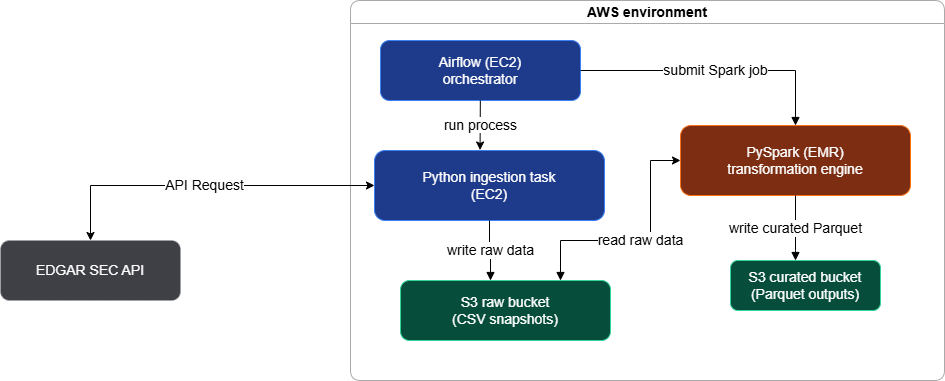
\includegraphics[width=0.9\textwidth]{diagrams/baseline_pipeline/arcitecture.png}
  \caption{Baseline runtime architecture showing orchestration,
  compute, and storage components.}
  \label{fig:baseline-architecture}
\end{figure}

\noindent
Continuous integration and deployment are automated through
GitHub~Actions. Figure~\ref{fig:baseline-cicd} illustrates the CI/CD
workflow: syntax checks precede infrastructure provisioning via
Terraform, after which the Airflow image---which embeds the DAGs---is
built, pushed to~GHCR, and redeployed to the EC2~host.

\begin{figure}[H]
  \centering
  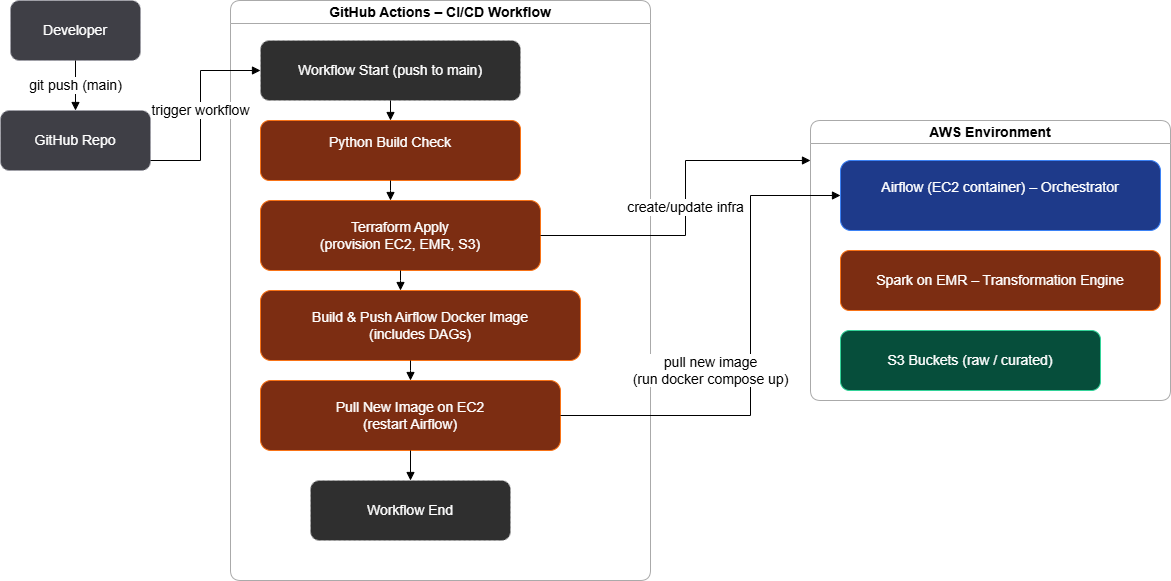
\includegraphics[width=0.9\textwidth]{diagrams/baseline_pipeline/ci_cd.png}
  \caption{CI/CD pipeline treated as a DAG within GitHub~Actions.}
  \label{fig:baseline-cicd}
\end{figure}

\section{Functionality}
\noindent
Figure~\ref{fig:baseline-dag} presents the Airflow~DAG that governs the
ETL workflow. A single linear sequence performs ingestion, submission
of Spark jobs, and post-run manifest recording.

\begin{figure}[H]
  \centering
  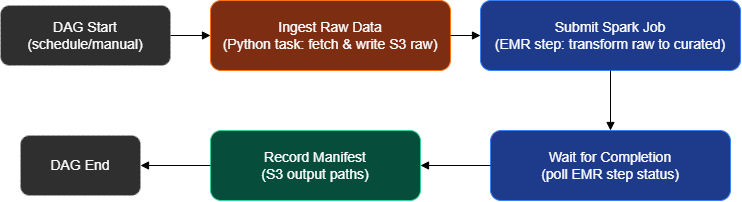
\includegraphics[width=0.85\textwidth]{diagrams/baseline_pipeline/airflow_dag.png}
  \caption{Baseline Airflow~DAG showing orchestration sequence.}
  \label{fig:baseline-dag}
\end{figure}

\noindent
Data moves through three primary stages (Figure~\ref{fig:baseline-data}).
The ingestion task fetches source files and stores them in the raw~S3
bucket. Spark reads these raw objects, enforces schema consistency,
cleans and deduplicates records, and writes Parquet datasets to the
curated bucket, partitioned by ingestion date. Each run emits a simple
manifest (\texttt{\_SUCCESS}) listing output paths for downstream
validation.

\begin{figure}[H]
  \centering
  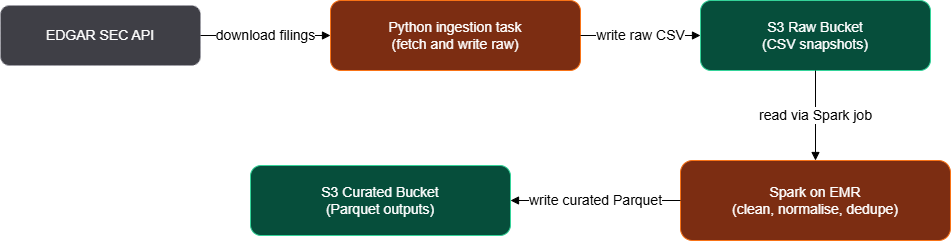
\includegraphics[width=0.85\textwidth]{diagrams/baseline_pipeline/data_path.png}
  \caption{Data path from ingestion to curated output in the baseline pipeline.}
  \label{fig:baseline-data}
\end{figure}

\section{Observed Gaps}
\noindent
While the baseline performs correctly, it lacks the controls required
for trustworthy audit evidence.

\paragraph{Lineage.}
Provenance is implicit in log files rather than captured as structured
metadata. No mapping links a specific input object, transformation
script, and output dataset.

\paragraph{Reproducibility.}
Environment state is defined by mutable container images. There is no
guarantee that a re-run reproduces prior results byte-for-byte, nor any
version pinning for dependencies or configuration.

\paragraph{Governance and Security.}
IAM policies are broad, and actions are not gated by review or policy
validation. Objects in S3 remain mutable and unsigned, and there is no
mechanism to detect tampering or verify artifact integrity.

\section{Summary}
\noindent
The baseline ETL pipeline demonstrates a functioning but ungoverned
data workflow. It provides consistent data movement from extraction to
curated storage, yet its assurance relies on convention rather than
design. The next chapter extends this model with explicit DevSecOps
controls---embedding lineage tracking, immutable evidence, and governed
infrastructure to meet auditability expectations.

\chapter{Proposed Architecture}

\section{Design Principles}
Outline the guiding principles of the proposed DevSecOps-integrated ETL system:
automation, immutability, traceability, reproducibility.

\section{High-Level Overview}
Provide an architectural diagram comparing baseline and proposed design.

\section{Core Components}
Explain each layer:
\begin{itemize}
    \item \textbf{Infrastructure as Code:} Terraform for provisioning.
    \item \textbf{Orchestration:} Airflow for controlled execution.
    \item \textbf{Security:} CI/CD checks, artifact signing, SAST/SCA.
    \item \textbf{Governance:} Immutable audit logs, metadata tracking.
\end{itemize}

\section{Integration with DevSecOps Practices}
Map the proposed pipeline to the DevSecOps lifecycle (plan → code → build → test → release → monitor).

\section{Expected Outcomes}
Summarize the architectural advantages for auditability and compliance.

\chapter{Prototype Implementation}
To be completed in Thesis B
% \section{Implementation Environment}
% List the environment setup:
% AWS EMR, EC2, S3, Docker, GitHub Actions, Terraform.

% \section{Toolchain Configuration}
% Show how tools interconnect (e.g., Airflow triggers Spark, CI/CD automates IaC).

% \section{Security and Governance Layers}
% Describe:
% \begin{itemize}
%     \item Hash signing of artifacts
%     \item Immutable logging mechanisms
%     \item Versioned configuration and audit history
% \end{itemize}

% \section{Demonstration}
% Summarize execution flow with example runs and screenshots.

% \section{Challenges}
% Briefly discuss debugging, integration issues, and trade-offs during build.

\chapter{Evaluation}
\label{ch:evaluation}
\noindent
This chapter evaluates the results reported in Chapter~\ref{ch:results}
against the requirements defined in Chapter~3. The results chapter shows what
the implemented architecture produced. This chapter considers whether those
outputs satisfy the requirements and whether they satisfy the auditability
definition used throughout the thesis.

The evaluation uses the definition from Chapter~2, where auditability is framed
as the designed capability of a system to allow its processes, controls, and
outcomes to be observed and verified by stakeholders. In that definition,
auditability is not a single log file or a general claim that monitoring
exists. It is made up of normativity, accountability, referentiality
infrastructure, reliability, and verifiability
\cite{weigand_auditability_2019}. The evaluation therefore asks whether the
implemented fields and artifacts make those dimensions visible in the system.

\section{Evaluation Approach}
\noindent
The assessment follows the R1--R5 requirement matrix from Chapter~3 and the
control matrix in the proposed-solution repository. Each requirement is
evaluated in three steps. First, the requirement is mapped back to the relevant
auditability dimensions. Second, the concrete evidence fields are identified.
Third, the observed result is judged against the requirement.

This approach deliberately treats the evidence artifacts as the primary object
of evaluation. A pipeline run is not considered auditable only because it
completed successfully. It is considered auditable if the produced dataset can
be linked to the governing change, release, infrastructure reference, runtime
code, quality decision, lineage event, and metadata record without manual log
collation.

\section{R1 Governance Accountability}
\noindent
R1 requires production-relevant changes to be linked to documented authority.
In Chapter~3 this requirement was tied to normativity and accountability.
Normativity is satisfied when the system records which governance rule or
change process applies to an action. Accountability is satisfied when the run
can be linked back to the actor, change, or approved release that authorised
the action.

\begin{table}[H]
  \centering
  \caption{R1 governance accountability evidence fields.}
  \label{tab:evaluation-r1-fields}
  \renewcommand{\arraystretch}{1.15}
  \begin{tabularx}{\textwidth}{@{}p{0.33\textwidth}X@{}}
    \toprule
    \textbf{Field or artifact} & \textbf{Evaluation role} \\
    \midrule
    \texttt{change\_ref} & Links the run to the governing change record. \\
    \texttt{release\_manifest\_ref} & Links the run to the approved release definition. \\
    \texttt{terraform\_state\_ref} & Links the run to the infrastructure state reference. \\
    \texttt{reference\_checks.change\_ref} & Records whether the change record resolved at runtime. \\
    \texttt{reference\_checks.release\_manifest\_ref} & Records whether the release manifest resolved at runtime. \\
    \texttt{reference\_checks.terraform\_state\_ref} & Records whether the infrastructure reference resolved at runtime. \\
    \texttt{source\_control.commit} & Links the release and run evidence to the source revision. \\
    Change record \texttt{change\_id} & Names the governed change, for example \texttt{EDGAR-1}. \\
    Release manifest \texttt{release\_id} & Names the governed release, for example \texttt{dev-edgar-v1}. \\
    \bottomrule
  \end{tabularx}
\end{table}

The requirement is demonstrated because the implemented run is not recorded as
an isolated Airflow execution. The run manifest contains the change, release,
and Terraform references, and the reference-check block records whether each
reference existed when the run evidence was produced. This means the run can be
read as an authorised operational event rather than only as a scheduled task.

The link to the auditability definition is direct. The \texttt{change\_ref} and
\texttt{release\_manifest\_ref} fields provide normativity because they record
the governing process that applied to the run. The source-control and release
fields provide accountability because they bind the run to a concrete change
record and code revision. The reference checks are important because they
prevent the evidence chain from merely naming authority; they record that the
named authority resolved.

\section{R2 Information Security Assurance}
\noindent
R2 requires deployable artifacts and configuration to be verified for integrity
and security before they are used. In Chapter~3 this was tied to reliability
and verifiability. Reliability is concerned with whether the evidence faithfully
represents the artifact that ran. Verifiability is concerned with whether an
independent reviewer can test the claim.

\begin{table}[H]
  \centering
  \caption{R2 information security assurance evidence fields.}
  \label{tab:evaluation-r2-fields}
  \renewcommand{\arraystretch}{1.15}
  \begin{tabularx}{\textwidth}{@{}p{0.33\textwidth}X@{}}
    \toprule
    \textbf{Field or artifact} & \textbf{Evaluation role} \\
    \midrule
    \texttt{code\_bundle.release\_manifest\_sha256} & Records the digest of the release manifest. \\
    \texttt{code\_bundle.artifacts.path} & Names each DAG or job artifact included in the bundle. \\
    \texttt{code\_bundle.artifacts.sha256} & Records a SHA-256 hash for each code artifact. \\
    \texttt{source\_control.repository} & Records the source repository used for the release. \\
    \texttt{source\_control.commit} & Records the source revision associated with the run. \\
    \texttt{attestation.provider} & Records the attestation provider expected by the evidence model. \\
    \texttt{attestation.subject\_digest} & Carries the subject digest used to bind provenance to the release artifact. \\
    GitHub Actions controls & Provide the CI/CD surface for linting, tests, policy checks, artifact upload, and attestation. \\
    \bottomrule
  \end{tabularx}
\end{table}

The requirement is demonstrated by the way the implementation records artifact
identity. The code bundle includes hashes for the DAG and the ingest,
transform, quality, and promotion jobs. These hashes make the run evidence more
reliable because an auditor can compare the recorded digest with the file that
is claimed to have run. The source-control fields then bind those artifacts to
the repository and commit.

The release provenance fields extend the same chain to the release context. The
evidence model records the provider, workflow, run, URL, and subject digest
fields needed to connect the release bundle to GitHub-native provenance. In
the implemented results, this requirement is evaluated through the demonstrated
source revision, run reference, release reference, and SHA-256 artifact hashes.

This satisfies the auditability definition because the security claim is
independently testable. An evaluator does not need to trust a written statement
that the correct files were used. The evaluator can inspect
\texttt{code\_bundle.artifacts.sha256}, compare it with the artifact contents,
and then follow \texttt{source\_control.commit} back to the release source.

\section{R3 Operational Risk Control}
\noindent
R3 requires the workflow to support reproducibility, recovery, and visibility
over operational state. In Chapter~3 this requirement was tied to
referentiality and reliability. Referentiality is satisfied when the run record
connects the output to its source, intermediate, and runtime records.
Reliability is satisfied when the recorded state is complete enough to support
replay and diagnosis.

\begin{table}[H]
  \centering
  \caption{R3 operational risk control evidence fields.}
  \label{tab:evaluation-r3-fields}
  \renewcommand{\arraystretch}{1.15}
  \begin{tabularx}{\textwidth}{@{}p{0.33\textwidth}X@{}}
    \toprule
    \textbf{Field or artifact} & \textbf{Evaluation role} \\
    \midrule
    \texttt{run\_id} & Identifies the specific governed execution. \\
    \texttt{pipeline\_id} & Identifies the pipeline definition that ran. \\
    \texttt{dataset\_date} & Identifies the dataset partition or business date. \\
    \texttt{source\_ref} & Records the source input used by the run. \\
    \texttt{raw\_outputs} & Records the raw payload and normalised raw output references. \\
    \texttt{curated\_outputs.curated\_uri} & Records the curated dataset produced by transformation. \\
    \texttt{quality\_result.status} & Records whether the quality gate passed. \\
    \texttt{gold\_write\_result} & Records the promoted gold table write result. \\
    \texttt{dataset\_version} & Records the stable output version used for reconstruction. \\
    \texttt{status} & Records the final run outcome. \\
    \texttt{completed\_at} & Records when the run evidence was finalised. \\
    \bottomrule
  \end{tabularx}
\end{table}

The requirement is demonstrated because the run manifest records enough state
to reconstruct how the output was created. It contains source, raw, curated,
quality, promotion, and dataset-version fields in a single evidence object.
This reduces operational risk because recovery no longer depends on reading
unrelated logs and guessing which task output should be trusted.

The manifest validator strengthens the result. For a successful run, the
validator requires a \texttt{dataset\_version}, a \texttt{gold\_write\_result},
and metadata references to the OpenMetadata run record, OpenMetadata dataset
record, OpenLineage event, and audit-chain path. It also requires reference
checks for the release, Terraform, and change references. A run is therefore
not merely successful because the final task completed. It is successful
because the evidence needed for reconstruction is present.

This maps to referentiality because each stage of the data path points to the
next stage. It maps to reliability because the system records the final status,
quality result, row-count evidence, and completion time together with the
output version. The result is a recovery-oriented run record rather than a
best-effort operational log.

\section{R4 Continuous Control Monitoring}
\noindent
R4 requires controls to run continuously and to produce evidence of their
outcomes. In Chapter~3 this requirement was tied to normativity and
accountability. Normativity is present when controls are embedded into the
workflow rather than applied after the fact. Accountability is present when the
result of each control decision is retained.

\begin{table}[H]
  \centering
  \caption{R4 continuous control monitoring evidence fields.}
  \label{tab:evaluation-r4-fields}
  \renewcommand{\arraystretch}{1.15}
  \begin{tabularx}{\textwidth}{@{}p{0.33\textwidth}X@{}}
    \toprule
    \textbf{Field or artifact} & \textbf{Evaluation role} \\
    \midrule
    \texttt{quality\_result.checks.curated\_output\_exists} & Records whether the curated output existed. \\
    \texttt{quality\_result.checks.schema\_matches\_contract} & Records whether the curated output matched the contract. \\
    \texttt{quality\_result.checks.row\_count\_gt\_zero} & Records whether the curated output contained records. \\
    \texttt{quality\_result.checks.required\_ids\_non\_null} & Records whether required identifiers were populated. \\
    \texttt{curated\_outputs.contract\_path} & Links the quality decision to the data contract. \\
    \texttt{reference\_checks} & Records whether governance references resolved before the run evidence was accepted. \\
    \texttt{metadata\_refs.openlineage\_event\_path} & Records where the lineage event evidence was written. \\
    \texttt{metadata\_refs.openmetadata\_run\_path} & Records where the run metadata evidence was written. \\
    \bottomrule
  \end{tabularx}
\end{table}

The requirement is demonstrated because the implementation converts controls
into runtime evidence. The quality result is not a general pass/fail statement;
it records named checks. The contract path also remains in the manifest, which
means the schema decision can be traced back to the exact contract used for the
check.

This matters for auditability because continuous monitoring must be observable.
If a quality or governance check only appears in a log line, the control is
difficult to test independently. In this implementation, the check result is a
field in the manifest and therefore becomes part of the same evidence chain as
the dataset version. The same pattern is used for governance references:
\texttt{reference\_checks} records whether the release manifest, Terraform
state reference, and change record resolved.

R4 is therefore satisfied within the implemented scope. The system demonstrates
that control execution and control outcome can be captured as structured
runtime evidence. The remaining production concern is scale and policy
coverage: more policies would be needed for a complete enterprise deployment,
but the architecture pattern is demonstrated.

\section{R5 End-to-End Evidence Chain}
\noindent
R5 is the strongest auditability requirement because it asks whether a promoted
dataset can be reconstructed from evidence without manual log collation. In
Chapter~3 this requirement was tied to referentiality and verifiability. It is
also the requirement that most directly tests the thesis claim.

\begin{table}[H]
  \centering
  \caption{R5 end-to-end evidence chain fields.}
  \label{tab:evaluation-r5-fields}
  \renewcommand{\arraystretch}{1.15}
  \begin{tabularx}{\textwidth}{@{}p{0.33\textwidth}X@{}}
    \toprule
    \textbf{Field or artifact} & \textbf{Evaluation role} \\
    \midrule
    \texttt{dataset\_version} & Starting point for reconstruction from the gold dataset. \\
    Audit-chain \texttt{manifest\_ref} & Resolves the dataset version to the run manifest. \\
    Audit-chain \texttt{release\_manifest\_ref} & Resolves the dataset version to the release manifest. \\
    Audit-chain \texttt{terraform\_state\_ref} & Resolves the dataset version to the infrastructure state reference. \\
    Audit-chain \texttt{change\_ref} & Resolves the dataset version to the governing change. \\
    Audit-chain \texttt{code\_bundle} & Carries the runtime code hashes into the reconstruction path. \\
    \texttt{metadata\_refs.audit\_chain\_path} & Records where the audit-chain artifact was written. \\
    OpenLineage \texttt{inputs} & Records source, raw, curated, and manifest lineage inputs. \\
    OpenLineage \texttt{outputs} & Records the gold-table lineage output and dataset version facet. \\
    OpenMetadata dataset \texttt{manifest\_ref} & Links the catalogue dataset record back to the run manifest. \\
    \bottomrule
  \end{tabularx}
\end{table}

The implemented result satisfies R5 because the dataset version
\texttt{9b5fd26a2005c02b} can be used as the first lookup key. From there, the
audit-chain artifact points to the run manifest. The run manifest then points
to the release manifest, Terraform state reference, change record, code bundle,
quality result, OpenLineage event, and OpenMetadata records.

This is the clearest link back to the auditability definition. Referentiality
is demonstrated because the evidence chain preserves the points of recording
for source data, raw output, curated output, manifest storage, metadata
publication, and gold promotion. Verifiability is demonstrated because those
links are materialised as fields and paths rather than implied by naming
convention. An evaluator can follow the fields directly:
\texttt{dataset\_version} to audit-chain file, audit-chain
\texttt{manifest\_ref} to run manifest, run manifest to governance references,
and metadata references to lineage and catalogue records.

R5 is therefore demonstrated because the system provides a structured
reconstruction path. The baseline pipeline could show that tasks ran and files
existed, but it did not bind the output to the change, release, infrastructure,
code, quality, lineage, and catalogue evidence in one chain. The proposed
architecture does.

\section{Evaluation Summary}
\noindent
The evaluation shows that the proposed architecture satisfies R1--R5 within
the implemented scope. More importantly, each requirement is satisfied in terms
of the auditability definition from Chapter~2. R1 and R4 demonstrate
normativity and accountability by recording the governing change, release,
reference checks, and control outcomes. R2 and R3 demonstrate reliability by
recording artifact hashes, source-control provenance, quality status, and
complete run state. R3 and R5 demonstrate referentiality by linking source,
raw, curated, manifest, metadata, and gold records. R2 and R5 demonstrate
verifiability because the recorded hashes, manifests, metadata references, and
audit-chain fields can be inspected independently.

The result is that auditability is implemented as a set of linked evidence
fields, not as a retrospective explanation. The proposed architecture therefore
meets the thesis objective: it improves ETL governance by making the authority,
integrity, runtime state, control decisions, and output reconstruction path
part of the delivery and execution workflow.

\chapter{Discussion}

\section{Summary of Findings}
Recap the main evaluation results and architectural improvements.

\section{Implications for Practice}
Explain how this approach could generalize to other regulated environments.

\section{Limitations}
Note scalability, data type constraints, or untested regulatory frameworks.

\section{Future Work}
Propose enhancements—e.g., integrating ML pipelines, policy-as-code frameworks, or extended logging.

\chapter{Conclusion}
\noindent
This thesis set out to answer the question:

\begin{quote}
How can a DevSecOps toolchain be designed to support ETL workflows in regulated
industries, enhancing auditability and data governance?
\end{quote}

The answer developed in this thesis is that DevSecOps can support governed ETL
when the delivery pipeline and the data pipeline are treated as one evidence
system. In the proposed architecture, a dataset is not only the output of an
Airflow run. It is the result of a governed change, an approved release, a
specific infrastructure state, a known code bundle, a quality decision, and a
recorded lineage path. Auditability is therefore designed into the workflow
rather than reconstructed after the workflow has already completed.

\section{Summary of Contributions}
\noindent
The first contribution of this thesis is the architecture itself. Chapter~5
presented a governed ETL architecture at escalating levels of detail, beginning
with the high-level system structure and moving through process maps, data
flows, metadata flows, and a worked execution path. This architecture extends a
standard Airflow and AWS-style ETL pipeline with change governance, release
manifests, policy checks, quality gates, lineage publication, metadata
records, and audit-chain artifacts.

The second contribution is the implemented prototype. The implementation used a
governed EDGAR pipeline to show how the architecture can be materialised in
code. The prototype produced run manifests, release references, change
references, code hashes, quality results, OpenLineage-style events,
OpenMetadata-compatible records, and audit-chain files. Although the
demonstration was intentionally scoped, it showed that a produced dataset
version can be traced back to the authority, code, infrastructure, and controls
that produced it.

The third contribution is the evaluation framework and requirement mapping.
Chapter~3 translated auditability and governance concerns into five system
requirements: governance accountability, information security assurance,
operational risk control, continuous control monitoring, and end-to-end
evidence chain. Chapter~7 then evaluated the prototype against these
requirements and linked each one back to the auditability dimensions of
normativity, accountability, referentiality, reliability, and verifiability.

\section{Findings}
\noindent
The main finding is that auditability improves when evidence is captured as
part of the delivery and runtime workflow. The baseline pipeline could produce
data and operational logs, but it did not bind the output to a complete
governance chain. The proposed architecture changed this by making the run
manifest and metadata artifacts central to the system.

The worked example in Chapter~6 demonstrated this point. Starting from the
example dataset version, the evidence chain could be followed to the
audit-chain artifact, run manifest, release manifest, Terraform reference,
change record, code hashes, quality decision, lineage event, and metadata
records. This does not remove the need for human judgement in an audit, but it
does change what the auditor is judging. Instead of assembling evidence from
unrelated logs and repository history, the auditor can inspect a structured
chain of fields and artifacts.

The evaluation also showed that the architecture is strongest when controls
produce evidence, not only decisions. A policy check that blocks deployment is
useful, but it becomes auditable when its result is retained and linked to the
release or run. A data contract is useful, but it becomes auditable when the
quality result records that the contract was checked before promotion. A
lineage record is useful, but it becomes stronger when it points to the same
dataset version and manifest as the rest of the evidence chain.

\section{Scope and Reflection}
\noindent
The demonstration was intentionally scoped around the evidence model. The EDGAR
pipeline and representative run were used to test whether a governed ETL system
could connect release identity, runtime state, quality evidence, lineage, and
metadata into a coherent audit chain. Production-scale reliability, multi-team
access-control behaviour, and long-term retention are operational extensions of
that same architecture rather than the focus of the evaluation.

The most important design trade-off is reliance on GitHub. GitHub is useful
because it brings source control, issues, pull requests, CI/CD, and release
automation close together. At the same time, that convenience concentrates
trust. The outages encountered during development made this risk clear. A
future production version of this architecture should split some of these
responsibilities across independent services so that audit evidence is not
dependent on one platform remaining continuously available and internally
consistent.

\section{Closing Remarks}
\noindent
This thesis demonstrates that DevSecOps can enhance ETL governance when it is
used to create durable evidence, not only automation. The proposed architecture
does not treat compliance as a final review step. It treats governance
references, release identity, code integrity, quality decisions, lineage, and
metadata as normal outputs of the pipeline.

For regulated environments, this matters because trust in data depends on more
than correct transformation logic. It depends on whether the organisation can
explain how the data was produced, who authorised the change, which controls
ran, and how the output can be reconstructed. The architecture developed in
this thesis provides a practical path toward that goal by making auditability a
designed property of the ETL system.




\appendix

\chapter{Abbreviations}
\label{chap:abbreviations}

\begin{tabbing}
APRA  \qquad\qquad \= Australian Prudential Regulation Authority\\
AWS   \> Amazon Web Services\\
CI/CD \> Continuous Integration / Continuous Delivery\\
CPG   \> Prudential Practice Guide (APRA)\\
CPS   \> Prudential Standard (APRA)\\
DAST  \> Dynamic Application Security Testing\\
DAG   \> Directed Acyclic Graph\\
DLC   \> Data Lifecycle\\
DSR   \> Design Science Research\\
ELT   \> Extract--Load--Transform\\
EMR   \> Elastic MapReduce\\
EC2   \> Elastic Compute Cloud\\
ETL   \> Extract--Transform--Load\\
GDPR  \> General Data Protection Regulation\\
GHCR  \> GitHub Container Registry\\
GitOps \> Git-based Operations\\
HIPAA \> Health Insurance Portability and Accountability Act\\
IaC   \> Infrastructure as Code\\
IAM   \> Identity and Access Management\\
IEEE  \> Institute of Electrical and Electronics Engineers\\
ISO   \> International Organization for Standardization\\
ML    \> Machine Learning\\
MLOps \> Machine Learning Operations\\
NIST  \> National Institute of Standards and Technology\\
PaC   \> Policy as Code\\
RBAC  \> Role-Based Access Control\\
S3    \> Simple Storage Service\\
SAST  \> Static Application Security Testing\\
SCA   \> Software Composition Analysis\\
SBOM  \> Software Bill of Materials\\
SDLC  \> Software Development Lifecycle\\
SSDF  \> Secure Software Development Framework\\
\end{tabbing}



\chapter{Baseline Pipeline Configuration}
% e.g. Terraform modules, Docker compose, Airflow DAGs
% \input{chapters/appendix_baseline.tex}

\chapter{Additional Evaluation Artifacts}
% e.g. extra tables, logs, screenshots
% \input{chapters/appendix_extra_eval.tex}

% ----------------------------- Bibliography --------------------------------

\bibliographystyle{IEEEtranS}
\bibliography{references}

\end{document}
